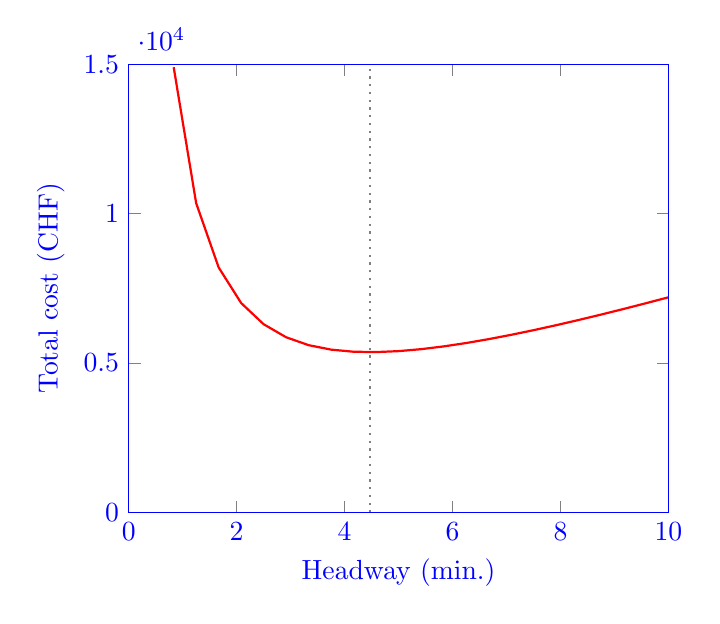
\begin{tikzpicture}[
  blue,
  declare function = {
    cost(\x) = \T * \r / \x ;
    waiting(\x) = \T * \x * \f / 2 ;
  }
]
  \def \T{60}
  \def \f{60}
  \def \r{200}
  \def \W{1/3}
  \begin{axis}[
      xlabel={Headway (min.)},
      ylabel={Total cost (CHF)},
      domain=0:10,
      xmin=0,
      xmax=10,
      ymin=0,
      ymax=15000,
      restrict y to domain=0:15000,
      axis on top,
    ]
    \addplot+[red, thick, no marks] {cost(x) + 20 * waiting(x) / 60}; 
    \draw[-, thick, dotted, gray] {
      ({(2 * \r / (\f * \W))^0.5}, 0) --
      ({(2 * \r / (\f * \W))^0.5}, \pgfkeysvalueof{/pgfplots/ymax})
    };
  \end{axis}
\end{tikzpicture}
